% !TEX program = xelatex
\documentclass[a4paper]{exam}
\usepackage{amsmath}
\usepackage{amsthm}
\usepackage[left=1.8cm,right=1.8cm,top=2.2cm,bottom=2.0cm]{geometry}
\usepackage{ctex}
\usepackage{enumerate}
\usepackage{fancyhdr}
\usepackage{xpatch}
\usepackage{graphicx} 
\usepackage{float} 
\usepackage{subfigure} 
\usepackage{amsfonts}
\usepackage{mathtools}
\usepackage{framed}
\usepackage{multicol}
\usepackage{listings,listings-rust}
\usepackage{minted}
\usepackage{hyperref}
\usepackage{biblatex}
\addbibresource{11-discussion.bib}
\usepackage{tikz}
\usetikzlibrary{automata,positioning}
\theoremstyle{definition}
\newtheorem*{solution*}{\textbf{Solution:}}
\newtheorem*{proof*}{\textbf{Proof:}}
\newtheorem{theorem}{Theorem}[subsection]
\newtheorem{definition}{Definition}[subsection]
\newtheorem{lemma}{Lemma}[subsection]
\makeatletter
% \usepackage{listings}% http://ctan.org/pkg/listings
\lstset{
  basicstyle=\ttfamily\tiny,
  mathescape,
}
\AtBeginDocument{\xpatchcmd{\@thm}{\thm@headpunct{.}}{\thm@headpunct{}}{}{}}
\makeatother

\pagestyle{fancy}
\renewcommand{\baselinestretch}{1.15}

\usepackage{paralist}
\let\itemize\compactitem
\let\enditemize\endcompactitem
\let\enumerate\compactenum
\let\endenumerate\endcompactenum
\let\description\compactdesc
\let\enddescription\endcompactdesc

% shorten footnote rule
\xpatchcmd\footnoterule
  {.4\columnwidth}
  {1in}
  {}{\fail}
  \pagestyle{fancy}
  \renewcommand{\baselinestretch}{1.15}
  \usepackage[scaled=0.85]{FiraMono}
  
  \lstset{basicstyle=\ttfamily, keywordstyle=\bfseries}
\title{CS 131 Compilers: Discussion 11: Garbage Collector, Trait vs. Concept and Codegen From Light IR}
\author{\textbf{杨易为}~~\textbf{吴凌云}~~\textbf{樊雨鑫} \\ \texttt{ \{yangyw,wuly2,fanyx\}@shanghaitech.edu.cn}}


\begin{document}
\maketitle
\section{C++ garbage collection}
C++ actually have runtime garbage collection, once put in 2008 and deprecated in 2013. If you use some of the implementation of C++, they have runtime resource garbage collector. Now, we only talk about the compile time resource allocation.
\subsection{Resource Acquisition Is Initialization}
RAII, which is the compiled time garbage collector first introduced in this \href{http://www.open-std.org/jtc1/sc22/wg21/docs/papers/2008/n2670.htm}{thread}, guarantees that the resource is available to any function that may access the object (resource availability is a class invariant, eliminating redundant runtime tests). It also guarantees that all resources are released when the lifetime of their controlling object ends, in reverse order of acquisition. Likewise, if resource acquisition fails (the constructor exits with an exception), all resources acquired by every fully-constructed member and base subobject are released in reverse order of initialization. This leverages the core language features (object lifetime, scope exit, order of initialization and stack unwinding) to eliminate resource leaks and guarantee exception safety. Another name for this technique is Scope-Bound Resource Management (SBRM), after the basic use case where the lifetime of an RAII object ends due to scope exit.

RAII can be summarized as follows:
\begin{enumerate}
  \item encapsulate each resource into a class, where
  \begin{enumerate}
    \item the constructor acquires the resource and establishes all class invariants or throws an exception if that cannot be done,
    \item the destructor releases the resource and never throws exceptions;
    
  \end{enumerate}
  \item always use the resource via an instance of a RAII-class that either
  \begin{enumerate}
    \item has automatic storage duration or temporary lifetime itself, or
\item    has lifetime that is bounded by the lifetime of an automatic or temporary object
  \end{enumerate}
  Move semantics make it possible to safely transfer resource ownership between objects, across scopes, and in and out of threads, while maintaining resource safety.
\\
  Classes with open()/close(), lock()/unlock(), or init()/copyFrom()/destroy() member functions are typical examples of non-RAII classes:

  \begin{minted}[mathescape, linenos]{c++}
#include <bits\stdc++.h>
class ResourceGuard{
  private:
    const std::string resource;
    enum RG{
      DEAD,
      LIVE,
      ACVITE
    }
  public:
    ResourceGuard(const std::string& res):resource(res){
      std::cout << "Acquire the " << resource << "." <<  std::endl;
    }
    ~ResourceGuard(){
      std::cout << "Release the "<< resource << "." << std::endl;
    }
};

int main() {
  ResourceGuard resGuard1{"memoryBlock1"};
  std::cout << "\nBefore local scope" << std::endl; {
    ResourceGuard resGuard2{"memoryBlock2"};
  }
  std::cout << "After local scope" << std::endl;
  std::cout << std::endl;
  std::cout << "\nBefore try-catch block" << std::endl;
  try {
      ResourceGuard resGuard3{"memoryBlock3"};
      throw std::bad_alloc();
  }   
  catch (std::bad_alloc& e){
      std::cout << e.what();
  }
  std::cout << "\nAfter try-catch block" << std::endl;
  std::cout << std::endl;
}
  \end{minted}
\end{enumerate}
\subsection{Modern C++ Resource Lifetime}
\subsubsection{string\_view}
The string "move" util to make the char like variable, whatever it come from, the fastest to deal with the memory reallocation. In function arg passing, \textbf{callers responsibility to ensure the data outlive the function call\cite{stringview}}.

\begin{minted}[mathescape, linenos]{c++}
#include <string>
std::size_t length(const std::string &s){
  return s.size();
}
int main(){
  return length("hello world! long string");
}
\end{minted}

We get the resources allocated on heap, no exception. it requires the function call's full prologue and epilogue.
\begin{minted}[mathescape, linenos]{assembly}
  length(std::__cxx11::basic_string<char, ;allocator statically calculated
    std::char_traits<char>, std::allocator<char> > const&):
  mov     rax, QWORD PTR [rdi+8]
  ret
main:
  push    r12
  xor     edx, edx
  push    rbx
  sub     rsp, 56
  lea     rdi, [rsp+16]
  lea     rbx, [rsp+32]
  mov     QWORD PTR [rsp+8], 24
  lea     rsi, [rsp+8]
  mov     QWORD PTR [rsp+16], rbx
  call    std::__cxx11::basic_string<char, 
    std::char_traits<char>, std::allocator<char> >::_
    M_create(unsigned long&, unsigned long)
  mov     rdx, QWORD PTR [rsp+8]
  movdqa  xmm0, XMMWORD PTR .LC0[rip] ;create a standard string using implicit conversion
  movabs  rcx, 7453010373645639783
  mov     QWORD PTR [rsp+16], rax
  mov     QWORD PTR [rsp+32], rdx
  movups  XMMWORD PTR [rax], xmm0 ; mov in an efficient way.
  mov     rdx, QWORD PTR [rsp+16]
  mov     QWORD PTR [rax+16], rcx
  mov     rax, QWORD PTR [rsp+8]
  mov     QWORD PTR [rsp+24], rax
  mov     BYTE PTR [rdx+rax], 0
  mov     rdi, QWORD PTR [rsp+16]
  mov     r12d, DWORD PTR [rsp+24]
  cmp     rdi, rbx
  je      .L3
  mov     rax, QWORD PTR [rsp+32]
  lea     rsi, [rax+1]
  call    operator delete(void*, unsigned long) ;resource deallocation
.L3:
  add     rsp, 56
  mov     eax, r12d
  pop     rbx
  pop     r12
  ret
.LC0:
  .quad   8031924123371070824
  .quad   7957697951841938546
\end{minted}
Instead, we can simply change $string$ to $string\_view$, which is very similar to $string$, but a view to it. And we still have the long string size at compile time.
\begin{minted}[mathescape, linenos]{assembly}
length(std::basic_string_view<char, std::char_traits<char> > const&):
  mov     rax, QWORD PTR [rdi]
  ret
main:
  mov     eax, 24
  ret
\end{minted}

\subsubsection{PMR}
PMR is for you to have a more sophisticated control of memory resources in C++, all about how, when and where to have your garbage may lie in, the design is something refer to channel in golang. Basically, it has at least 4 pros:
\begin{enumerate}
  \item Fewer calls to new and delete
  \item Reduced thread contention
  \item Reduced false sharing
  \item Reduced memory diffusion
\end{enumerate} 
In PMR, you can allocate a monotonic buffer resource or local thread stack resource. This solve the following 3 problems, just let the memory allocation unique to one thread. You can get a test of this \href{https://github.com/lefticus/cpp_weekly/blob/master/PMR/performance_tests.cpp}{code}
\subsubsection{\href{https://www.oreilly.com/library/view/effective-modern-c/9781491908419/ch04.html}{smart pointer}}
Use \texttt{std::unique\_ptr} for exclusive-ownership resource management. \\
\begin{minted}[mathescape, linenos]{c++}
  class Investment { … };
  class Stock:
    public Investment { … };
  class Bond:
    public Investment { … };
  class RealEstate:
    public Investment { … };
\end{minted} \\
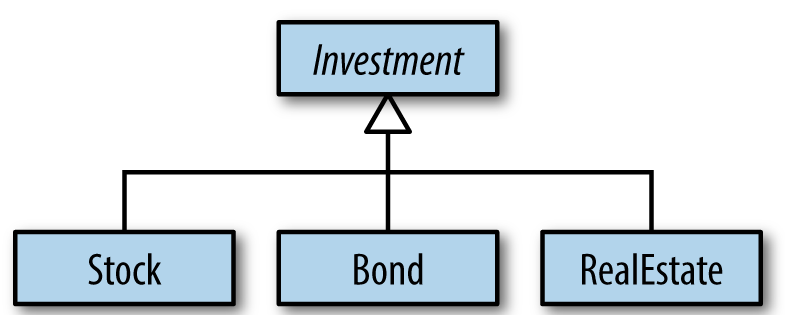
\includegraphics[width=10cm]{img/oop.png}

A factory function for such a hierarchy typically allocates an object on the heap and returns a pointer to it, with the caller being responsible for deleting the object when it’s no longer needed. That’s a perfect match for std::unique\_ptr, because the caller acquires responsibility for the resource returned by the factory (i.e., exclusive ownership of it), and the std::unique\_ptr automatically deletes what it points to when the std::unique\_ptr is destroyed. A factory function for the Investment hierarchy could be declared like this:

\begin{minted}[mathescape, linenos]{c++}
  template<typename... Ts>              // return std::unique_ptr
  std::unique_ptr<Investment>           // to an object created
  makeInvestment(Ts&&... params);       // from the given args

  auto delInvmt = [](Investment* pInvestment)       // custom
  {                                 // deleter
    makeLogEntry(pInvestment);      // (a lambda
    delete pInvestment;             // expression)
  };

template<typename... Ts>                          // revised
std::unique_ptr<Investment, decltype(delInvmt)>   // return type
makeInvestment(Ts&&... params) {
  std::unique_ptr<Investment, decltype(delInvmt)> // ptr to be
  pInv(nullptr, delInvmt);                      // returned

  if ( /* a Stock object should be created */ ) 
    pInv.reset(new Stock(std::forward<Ts>(params)...));
  else if ( /* a Bond object should be created */ ) 
    pInv.reset(new Bond(std::forward<Ts>(params)...));
  else if ( /* a RealEstate object should be created */ ) 
    pInv.reset(new RealEstate(std::forward<Ts>(params)...));

  return pInv;
}
\end{minted}

\subsubsection{Use std::shared\_ptr for shared-ownership resource management.}
\begin{enumerate}
  \item std::shared\_ptrs are twice the size of a raw pointer, because they internally contain a raw pointer to the resource as well as a raw pointer to the resource’s reference count.2

  \item Memory for the reference count must be dynamically allocated. Conceptually, the reference count is associated with the object being pointed to, but pointed-to objects know nothing about this. They thus have no place to store a reference count. (A pleasant implication is that any object—even those of built-in types—may be managed by std::shared\_ptrs.) Item 21 explains that the cost of the dynamic allocation is avoided when the std::shared\_ptr is created by std::make\_shared, but there are situations where std::make\_shared can’t be used. Either way, the reference count is stored as dynamically allocated data.
  
  \item Increments and decrements of the reference count must be atomic, because there can be simultaneous readers and writers in different threads. For example, a std::shared\_ptr pointing to a resource in one thread could be executing its destructor (hence decrementing the reference count for the resource it points to), while, in a different thread, a std::shared\_ptr to the same object could be copied (and therefore incrementing the same reference count). Atomic operations are typically slower than non-atomic operations, so even though reference counts are usually only a word in size, you should assume that reading and writing them is comparatively costly.
\end{enumerate}

\begin{minted}[mathescape, linenos]{c++}
auto loggingDel = [](Widget *pw)        // custom deleter
  {                     // (as in Item 18)
    makeLogEntry(pw);
    delete pw;
  };

std::unique_ptr<                        // deleter type is
 Widget, decltype(loggingDel)          // part of ptr type
 > upw(new Widget, loggingDel);

std::shared_ptr<Widget>                 // deleter type is not
 spw(new Widget, loggingDel);          // part of ptr type
\end{minted}
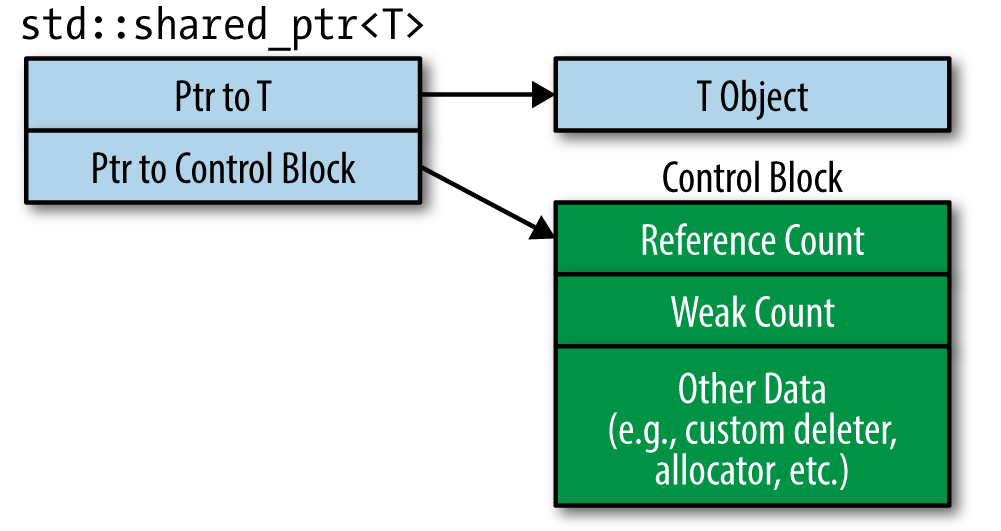
\includegraphics[width=10cm]{img/shared_ptr.png}

\subsubsection{Use std::weak\_ptr for std::shared\_ptr-like pointers that can dangle.}

As a final example of std::weak\_ptr’s utility, consider a data structure with objects A, B, and C in it, where A and C share ownership of B and therefore hold std::shared\_ptrs to it:

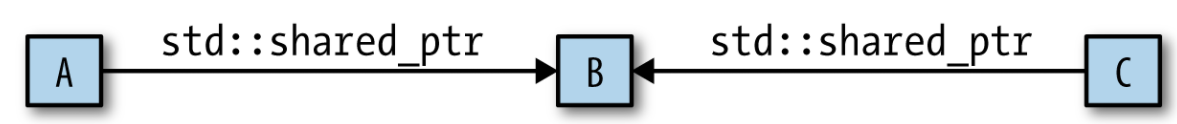
\includegraphics[width=10cm]{img/weak_ptr.png}\\
Suppose it’d be useful to also have a pointer from B back to A. What kind of pointer should this be?
\begin{enumerate}
  \item A raw pointer. With this approach, if A is destroyed, but C continues to point to B, B will contain a pointer to A that will dangle. B won’t be able to detect that, so B may inadvertently dereference the dangling pointer. That would yield undefined behavior.

  \item A std::shared\_ptr. In this design, A and B contain std::shared\_ptrs to each other. The resulting std::shared\_ptr cycle (A points to B and B points to A) will prevent both A and B from being destroyed. Even if A and B are unreachable from other program data structures (e.g., because C no longer points to B), each will have a reference count of one. If that happens, A and B will have been leaked, for all practical purposes: it will be impossible for the program to access them, yet their resources will never be reclaimed.
  
  \item A std::weak\_ptr. This avoids both problems above. If A is destroyed, B’s pointer back to it will dangle, but B will be able to detect that. Furthermore, though A and B will point to one another, B’s pointer won’t affect A’s reference count, hence can’t keep A from being destroyed when std::shared\_ptrs no longer point to it.
\end{enumerate}
Potential use cases for std::weak\_ptr include caching, observer lists, and the prevention of std::shared\_ptr cycles.
\subsection{Runtime Garbage Collector}
An object instance $x$ is \textbf{Reachable} on heap iff some variable (either in register or in memory) points to $x$, or another Reachable object $y$ contains a pointer to $x$. Unreachable objects are called \textbf{Garbage}, and is desired to get recycled by automatic memory management.

The concept of Reachability is sound (safe) but not complete, since Unreachable objects are definitely useless, but not all Reachable objects will be used later.

A example snapshot of the heap during execution can be:

\begin{enumerate}
    \item e.g.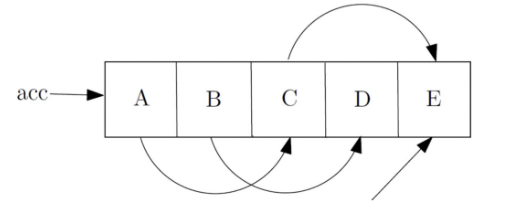
\includegraphics[width=5cm]{img/reachability.png}
    \item Arraws indicates refernce pointings
    \item \texttt{Roots} includes all references coming form outside the heap (in \texttt{ACC} or on stack)
\end{enumerate}
Various strategies of doing Garbage Collection (GC) exist. Three simple strategies are introduced below.
\subsubsection{Mark \& Sweep}
When running out of memory conduct the following two stages:
\begin{enumerate}
    \item Start from Roots, mark all Reachable objects
\item Erase all Unreachable objects, while leaving Reachable ones unmoved
\end{enumerate}
Will fragment the memory, but no need to update pointers since unmoved.
\subsubsection{Stop \& Copy}
Memory is partitioned into two equal areas $S_{o l d}, S_{n e w}$, while $S_{\text {old }}$ is the one under use currently. When $S_{\text {old }}$ runs full, copy all Reachable objects to the beginning of $S_{n e w}$, and the rest of the memory is then considered free.
\begin{enumerate}
    \item e.g.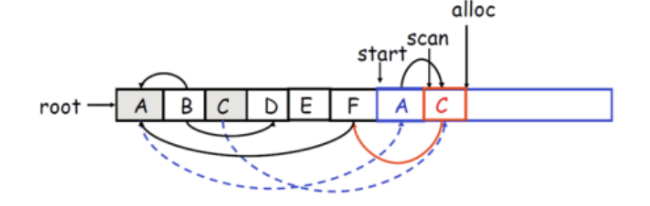
\includegraphics[width=5cm]{img/stop_and_copy.png}
    \item Notice the order:
    \begin{enumerate}
        \item First copy a Root $A$
 \item Follow its out-going reference to $C$, сopy $C$
  \item Update the pointer in $A$
 \item Repeat, starting from $C$
 \item If a referenced child is already copied, simply update the pointer
    \end{enumerate}
 
\end{enumerate}
Avoids fragmentations, but is time- and memory-expensive, since pointers need to be updated, and only half of memory is available.
\subsubsection{Ref Coundting}
Reference Counting (RC) is a dynamic GC strategy. We denote $r c(x)$ as the Reference Count of object $x$, where:
\begin{enumerate}
    \item A new object $x$ has $r c(x)=1$
\item After each assignment $x \leftarrow y, r c(x)-1, r c(y)+1$
\item When a variable $a$ (pointing to $x$ ) goes out out Scope, $r c(x)-1$
\item Free 0 -referenced objects at certain times
\end{enumerate}
Easy to implement, but very slow, and CANNOT handle circular references (where each $r c>0$, but the whole group is not Reachable).
\subsubsection{Case Study: Go GC}
There are two main types of garbage collection algorithms, namely, tracing garbage collection algorithm and reference counting method. The three-color tagging method is one of the tracing garbage collection algorithms.

The core idea of tracing algorithm is to determine whether an object is reachable or not, because once the object is not reachable, it can be immediately reclaimed by GC. So how do we determine whether an object is reachable or not? The first step is to find all global variables and variables in the current function stack and mark them as reachable. In the second step, starting from the data already marked, further mark the variables they are accessible to, and so on, in the technical terminology called passing closures.

The Go language garbage collector has been evolving since day one, except for a few versions without major updates, almost every minor release improves the performance of garbage collection, and along with the performance improvement is the complexity of the garbage collector code, \href{https://draveness.me/golang/docs/part3-runtime/ch07-memory/golang-garbage-collector/}{this} section will analyze the evolution of the garbage collector starting from the Go language v1.0 version.
\subsection{Three color label algorithm}
\begin{figure}[htbp]
  \centering
  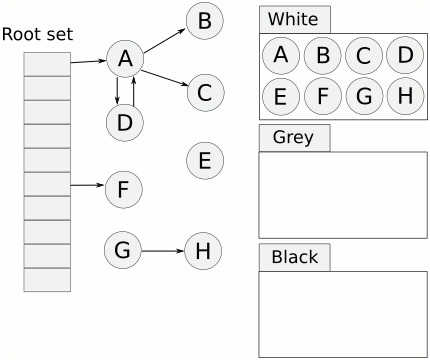
\includegraphics[width=5cm]{./img/tri_1.png}
  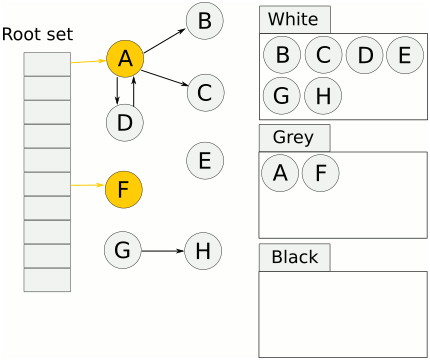
\includegraphics[width=5cm]{./img/tri_2.png}
  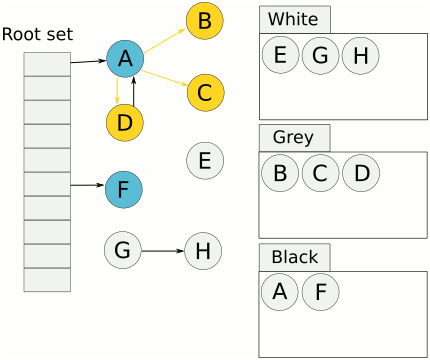
\includegraphics[width=5cm]{./img/tri_3.png}
  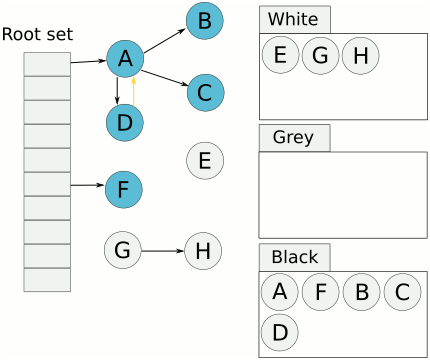
\includegraphics[width=5cm]{./img/tri_4.png}
  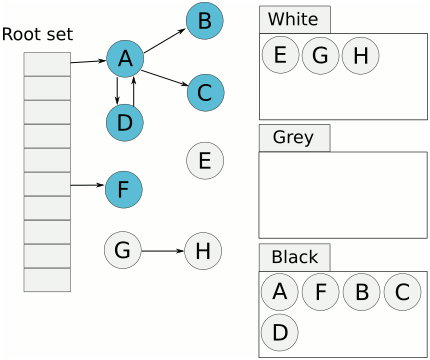
\includegraphics[width=5cm]{./img/tri_5.png}
  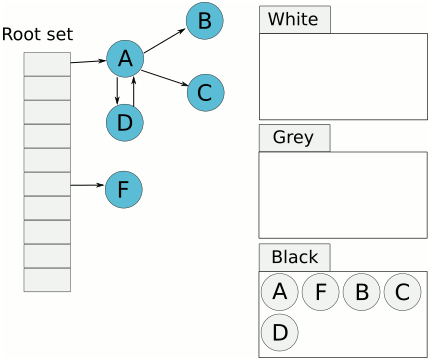
\includegraphics[width=5cm]{./img/tri_6.png}
  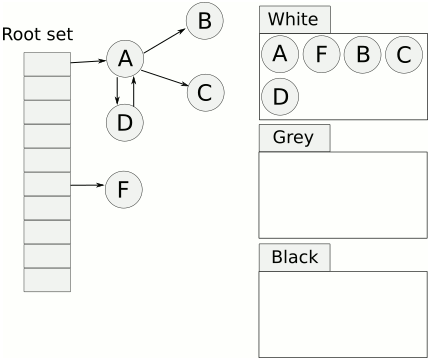
\includegraphics[width=5cm]{./img/tri_7.png}
\end{figure}
\section{Trait vs. Concept}
We may compare with the trait systems in rust or scala with the modern c++'s concepts, both of them are compile time check for the function and variable you defined. Since in many programer's mind, the Inheritance and combination is deprecated. See the following example:
\begin{minted}[mathescape, linenos]{c++}
class IStream {
public:
    virtual ~IStream() {}
public:
    virtual size_t read(std::uint8_t* buffer, size_t capacity) = 0;
    virtual size_t write(const std::uint8_t* buffer, size_t size) = 0;
};

class Console : public IStream { ... };
class FileStream : public IStream { ... };

void some_algorithm(IStream& stream) {
    std::uint8_t buffer[BUFFER_SIZE];
    size_t read = stream.read(buffer, sizeof(buffer));
    // do something
}
\end{minted}
This is a typical example of dynamic (runtime) polymorphism. It is implemented by adding a field (vptr) at the beginning of each Console and FileStream object, which points to a table of virtual functions. When the corresponding read and write methods are used, this virtual function table pointer is found first, then the corresponding function pointer is found, and then the corresponding function call is made.

Here the overhead of virtual functions is introduced, so for C++, which boasts zero-cost abstraction, this is costly, so another option is introduced.

\subsection{Template and overload}

\begin{minted}[mathescape, linenos]{c++}
class Console { ... };
class FileStream { ... };

template < class TStream >
void some_algorithm(TStream& stream) {
    std::uint8_t buffer[BUFFER_SIZE];
    size_t read = stream.read(buffer, sizeof(buffer));
    // do something
}
\end{minted}
Here you can see that since the template is directly connected to the corresponding function by overloading during the compilation stage when the template is expanded, the dispatch (dispatch) is done at the compilation stage, so it is called static dispatch, which eliminates the overhead of virtual functions.

\subsubsection{Problems faced by polymorphism in C++}
\begin{enumerate}
\item When using static dispatch, due to the complete reliance on overloading, when writing the corresponding code, it is difficult to ensure that your class completely implements the requirements of the calling code, plus the use of deep templates, resulting in error messages that are very difficult to read; to solve this problem the C++ standard committee added the concept of concepts to the C++ 20 standard, which can explicitly propose constraints\cite{cppref}.
\item When using dynamic dispatching, due to the presence of vptr, it destroys the memory structure of the object itself, which can be called a significant problem when your object also needs to interact with other libraries (especially those written in C).
\item Since C++ is a very mature language, and concept is a concept that will be added in the next standard, the constraints for static and dynamic derivation are completely different syntaxes, and for the same constraint, if we need to use both static and dynamic derivation, we must write it twice (once for virtual base classes and once for concepts).
\end{enumerate}

\subsubsection{Inheritance is the deepest coupling}
The hazards of coupling were described above, and inheritance is the deepest coupling. Because in the inheritance relationship, the parent class will expose its implementation to the child class, and the child class will no longer be interface-oriented, but rather programming-oriented implementation of the parent class.

In the field of object-oriented, there is a classic book, of course, is the "Gang of Four" "Design Patterns". At the beginning of the book, it is clearly stated that "combination is better than inheritance", which is the same reason.

\subsection{Solution in Rust Trait}
\begin{minted}[mathescape, linenos]{rust}
trait Stream {
    fn read(&mut self, buffer: &mut [u8]) -> usize;
    fn write(&mut self, buffer: &[u8]) -> usize;
}

struct Console;
struct FileStream;

impl Console { ... }
impl FileStream { ... }

impl Stream for Console {
   fn read(&mut self, buffer: &mut [u8]) -> usize { ... }
   ...
}

impl Stream for FileStream { ... }

fn some_algorithm_dynamic(stream: &mut dyn Stream) {
    let mut buffer = [0u8; BUFFER_SIZE];
    stream.read(&mut buffer);
    // do something
}

fn some_alogrithm_static<T : Stream>(stream: &mut T) {
    let mut buffer = [0u8; BUFFER_SIZE];
    stream.read(&mut buffer);
    // do something
}
\end{minted}
Comparing the C++ code, we can see that
\begin{enumerate}
    \item  For static dispatching, I can provide constraints directly in the form of T: Stream, requiring that the type parameter T of this generic function implements the trait Stream.
   \item When it comes to dynamic dispatching, Rust chooses a different way to implement it. Let's focus on the argument type of the function some\_algorithm\_dynamic function. It is \texttt{\&mut dyn} Stream, indicating that it is a variable trait object of type Stream. unlike C++, in Rust the virtual function table pointer is not placed into the object's memory structure, but is passed in as a field of the trait object, a fat pointer object (think of the trait object as a structure with 2 fields, one pointing to the object and the other to the vtable).
   \item The semantics of trait in Rust unifies the need for both static and dynamic dispatching; you only need to declare it once and implement it once to achieve static and dynamic dispatching according to your needs.
\end{enumerate}

\subsection{Use Concept to Rewrite Trait}
Here's an example trait to use Oracle to access to impled struct with bounded type and trait.
\begin{minted}[mathescape, linenos]{rust}
/// Oracle for feasibility problems
pub trait OracleFeas {
    type ArrayType;
    // f64 for 1D; ndarray::Array1<f64> for general
    type CutChoices;
    // f64 for single cut; (f64, Option<f64) for parallel cut
    fn assess_feas(&mut self, x: &Self::ArrayType) -> Option<(Self::ArrayType, Self::CutChoices)>;
}

/// Oracle for optimization problems
pub trait OracleOptim {
    type ArrayType;
    // f64 for 1D; ndarray::Array1<f64> for general
    type CutChoices;
    // f64 for single cut; (f64, Option<f64) for parallel cut
    fn assess_optim(
        &mut self,
        x: &Self::ArrayType,
        t: &mut f64,
    ) -> ((Self::ArrayType, Self::CutChoices), bool);
}

/// Oracle for quantized optimization problems
pub trait OracleQ {
    type ArrayType;
    // f64 for 1D; ndarray::Array1<f64> for general
    type CutChoices;
    // f64 for single cut; (f64, Option<f64) for parallel cut
    fn assess_q(
        &mut self,
        x: &Self::ArrayType,
        t: &mut f64,
        retry: bool,
    ) -> (
        (Self::ArrayType, Self::CutChoices),
        bool,
        Self::ArrayType,
        bool,
    );
}

pub trait OracleBS {
    fn assess_bs(&mut self, t: f64) -> bool;
}
\end{minted}
We can rewrite it into concept:
\begin{minted}[mathescape, linenos]{c++}
template<typename T> using ArrayType = typename T::ArrayType;
template<typename T> using CutChoices = typename T::CutChoices;
template<typename T> using Cut = std::pair<ArrayType<T>, CutChoices<T>>;
template<typename T> using RetQ = std::tuple<Cut<T>, bool, ArrayType<T>, bool>;


template<class Oracle>
concept OracleFeas = requires(Oracle omega, const ArrayType<Oracle> &x) {
    typename Oracle::ArrayType;   // double for 1D; ndarray::Arr1 for general
    typename Oracle::CutChoices;  // double for single cut; (double, Option<double) for parallel cut
    { omega.assess_feas(x) } -> std::convertible_to<std::optional<Cut<Oracle>>>;
};

template<class Oracle>
concept OracleOptim = requires(Oracle omega, const ArrayType<Oracle> &x, double &t) {
    typename Oracle::ArrayType;   // double for 1D; ndarray::Arr1 for general
    typename Oracle::CutChoices;  // double for single cut; (double, Option<double) for parallel cut
    { omega.assess_optim(x, t) } -> std::convertible_to<std::pair<Cut<Oracle>, bool>>;
};

template<class Oracle>
concept OracleQ = requires(Oracle omega, const ArrayType<Oracle> &x, double &t, bool retry) {
    typename Oracle::ArrayType;   // double for 1D; ndarray::Arr1 for general
    typename Oracle::CutChoices;  // double for single cut; (double, Option<double) for parallel cut
    { omega.assess_q(x, t, retry) } -> std::convertible_to<RetQ<Oracle>>;
};

template<class Oracle>
concept OracleBS = requires(Oracle omega, double &t) {
    { omega.assess_bs(t) } -> std::convertible_to<bool>;
};

template<class Space, typename T>
concept SearchSpace = requires(Space ss, const std::pair<ArrayType<Space>, T> &cut) {
    typename Space::ArrayType;  // double for 1D; ndarray::Arr1 for general
    { ss.xc() } -> std::convertible_to<ArrayType<Space>>;
    { ss.update(cut) } -> std::convertible_to<std::pair<CutStatus, double>>;
};
\end{minted}

\section{Codegen in Light IR}
\subsection{RISCV Spec}
定义详见 [RISCV Spec](https://riscv.org/technical/specifications/), [RVV](https://github.com/riscv/riscv-v-spec).

\subsection{后端介绍}

\subsection{对寄存器和地址的抽象}
值的地址。
\begin{minted}[mathescape,linenos]{c++}
class Value {
public:
    virtual constexpr bool is_reg() const = 0;
    virtual constexpr bool is_constant() const = 0;
    virtual constexpr bool has_shift() const = 0;
    virtual constexpr string_view get_name() const = 0;
};
\end{minted}
对寄存器的抽象
\begin{minted}[mathescape,linenos]{c++}
class Reg : public Value {
    int id;
public:
    explicit Reg(int id) : id(id) {
        if (id < 0 || id > max_reg_id) {
            LOG(ERROR) << "Invalid Reg ID!";
            abort();
        }
    }
    bool is_reg() const override { return true; }
    bool is_constant() const override { return false; }
    bool has_shift() const override { return false; }
    int getID() const { return this->id; }
    string_view get_name() const override { return reg_name[id]; }
    constexpr bool operator<(const Reg &rhs) const { return this->id < rhs.id; }
    constexpr bool operator==(const Reg &rhs) const { return this->id == rhs.id; }
    constexpr bool operator!=(const Reg &rhs) const { return this->id != rhs.id; }
};
class RegShift : public Value {
public:
    enum ShiftType { lsl, lsr, asl, asr };
private:
    int id;
    int shift;
    ShiftType _t;
}
\end{minted}
callee \& caller saved \& temporary \&& general register
\begin{minted}[mathescape,linenos]{c++}
const vector<InstGen::Reg> caller_save_regs =
  {InstGen::Reg(1),  InstGen::Reg(5),  
  InstGen::Reg(6),  InstGen::Reg(7),
  InstGen::Reg(10), InstGen::Reg(11), 
  InstGen::Reg(12), InstGen::Reg(13),
  InstGen::Reg(14), InstGen::Reg(15), 
  InstGen::Reg(16), InstGen::Reg(17),
  InstGen::Reg(28), InstGen::Reg(29),
  InstGen::Reg(30), InstGen::Reg(31)};
const vector<InstGen::Reg> callee_save_regs = 
  {InstGen::Reg(2),  InstGen::Reg(8),
  InstGen::Reg(9),  InstGen::Reg(18),
  InstGen::Reg(19), InstGen::Reg(20), 
  InstGen::Reg(21), InstGen::Reg(22),
  InstGen::Reg(23), InstGen::Reg(24), 
  InstGen::Reg(25), InstGen::Reg(26),
  InstGen::Reg(27)};
const vector<InstGen::Reg> allocate_regs = 
  {InstGen::Reg(10), InstGen::Reg(11), 
  InstGen::Reg(12), InstGen::Reg(13),
  InstGen::Reg(14), InstGen::Reg(15), 
  InstGen::Reg(16), InstGen::Reg(17)};
const vector<InstGen::Reg> temp_regs = 
  {InstGen::Reg(5),  InstGen::Reg(6),  
  InstGen::Reg(7), InstGen::Reg(28),
  InstGen::Reg(29), InstGen::Reg(30), 
  InstGen::Reg(31)};
\end{minted}
地址
\begin{minted}[mathescape,linenos]{c++}
class Addr {
    Reg reg;
    int offset;
    string str;
public:
    explicit Addr(Reg reg, int offset) : reg(std::move(reg)), offset(offset) {}
    Addr(string str) : str(std::move(str)), reg(Reg(0)), offset(0) {}
    Addr(string_view str) : str(str.begin(), str.end()), reg(Reg(0)), offset(0) {}
    Addr(const char *str) : str(str), reg(Reg(0)), offset(0) {}
    Reg getReg() const { return this->reg; }
    int getOffset() const { return this->offset; }
    string_view get_name() const;
};
\end{minted}
一个名字的 Label
\begin{minted}[mathescape,linenos]{c++}
class Label {
    string label;
    int offset;
public:
    explicit Label(string label, int offset) : label(move(label)), offset(offset) {}
    explicit Label(string label) : label(move(label)), offset(0) {}
    string_view get_name() const { return fmt::format("{}+{}", label, offset); }
};
\end{minted}
Heap Size/ L1 Size/ L2 Size
\subsection{寄存器分配}

本项目使用图着色法

Interface Graph图中的每个节点代表某个变量的活跃期或生存期(Live range)。活跃期定义是从变量第一次被定义(赋值)开始,到它下一次被赋值前的最后一次被使用为止。两个节点之间的边表示这两个变量活跃期因为生命期(lifetime)重叠导致互相冲突或干涉。一般说来,如果两个变量在函数的某一点是同时活跃(live)的,它们就相互冲突,不能占有同一个寄存器。

https://www.zhihu.com/question/56005792/answer/147558407

图着色算法:https://web.eecs.umich.edu/~mahlke/courses/583f12/reading/chaitin82.pdf

线性扫描算法:https://www2.seas.gwu.edu/~hchoi/teaching/cs160d/linearscan.pdf

偏向CISC指令集的Second chance binpacking算法

SSA形式带来的优点就是能有效的降低单个interval的长度,这在CISC指令集计算机中会非常有效。同时,充分利用SSA形式的IR的稀疏特性,避免迭代式的liveness analysis。有效的降低时间复杂度。

http://citeseerx.ist.psu.edu/viewdoc/download?doi=10.1.1.162.2590&rep=rep1&type=pdf

\printbibliography

\end{document}
